\begin{filecontents*}{\jobname.xmpdata}
  \Title{Your Thesis Title}
  \Author{Matthew Asher Bardin}
  \Keywords{comma, separated, keywords}
  \Date{2015-05-15}
  \Language{en-US}
\end{filecontents*}
%
\documentclass[doublespacing]{lsuthesis}
%% To experiment with using a different document class, such as the ``book''
%% class, comment-out the prior line and uncomment the next line.
%\documentclass[10pt,oneside]{book}

%% Specify additional LaTeX packages you need.
%\usepackage{graphicx}
%\usepackage{amsmath}
%\usepackage{amsthm}
\usepackage{pdfpages}
\usepackage{url}
\usepackage{lsutitle}
\title{CYBERINET: INTEGRATED SEMI-MODULAR SENSORS FOR THE
COMPUTER-AUGMENTED CLARINET}
\thesistype{Dissertation}
\department{The School of Music}
\soughtdegree{Doctor of Philosophy}
\author{Matthew Asher Bardin}
\degrees{B.M., Stetson University, 2017\\
  M.M., The Boston Conservatory at Berklee, 2019}
\graduationdate{August 2023}


\begin{document}

%% The command ``\frontmatter'' switches to lowercase roman page numbers and
%% unnumbered chapter headings without the word ``Chapter''.
\frontmatter

\maketitle


%% The following ``Copyright'' page is optional. You have inherent copyright
%% on anything you create, even if you choose not to include a copyright
%% notice. But if you choose to also formally register your copyright with
%% the Library of Congress, then a centered copyright notice should follow
%% the title page.
\begin{centeredpage}
\copyright\ 2023\\
Matthew Asher Bardin
\end{centeredpage}  


%% The following ``Dedication'' page is optional.
% \begin{centeredpage}
% The dedication goes here. remove these lines if I don't have one
% \end{centeredpage}


%% The following ``Epigraph'' page is optional.
% \begin{centeredpage}
% \epigraph{All these months I’ve been trying to find find a pattern. Trying not so much to draw hands as gestures. Not so much faces as the expressions of people.}{--Vincent Van Gogh}

% \end{centeredpage}


\chapter{Acknowledgments}

First, I would like to thank my family. Without their continued support, I would not have been able to make it into graduate school, let alone be finishing my dissertation project. Thank you from the bottom of my heart Mom, Dad, Michael, Melanie, and everyone else. 

I would also like to thank my various professors and mentors that I have had the pleasure of working with over the past decade. From building a general approach to music and technology in my undergraduate studies, to finding my passion while finishing my Master’s degree in Boston, to the guidance I received on this project; the advice I have received from these people has helped me to not only build a strong knowledge base, but achieve the confidence to present my work and my art to the world. [name drop here?]

Lastly, I would like to thank my cat, Bean. Regardless of whether she was in the way; she always made a spot on my desk to join me while I was writing. When in doubt, I would always defer to her expert opinion on any matters related to eat-scratches, pets, and wet food. Thank you, Bean.

\vspace{10mm}

\begin{center}
    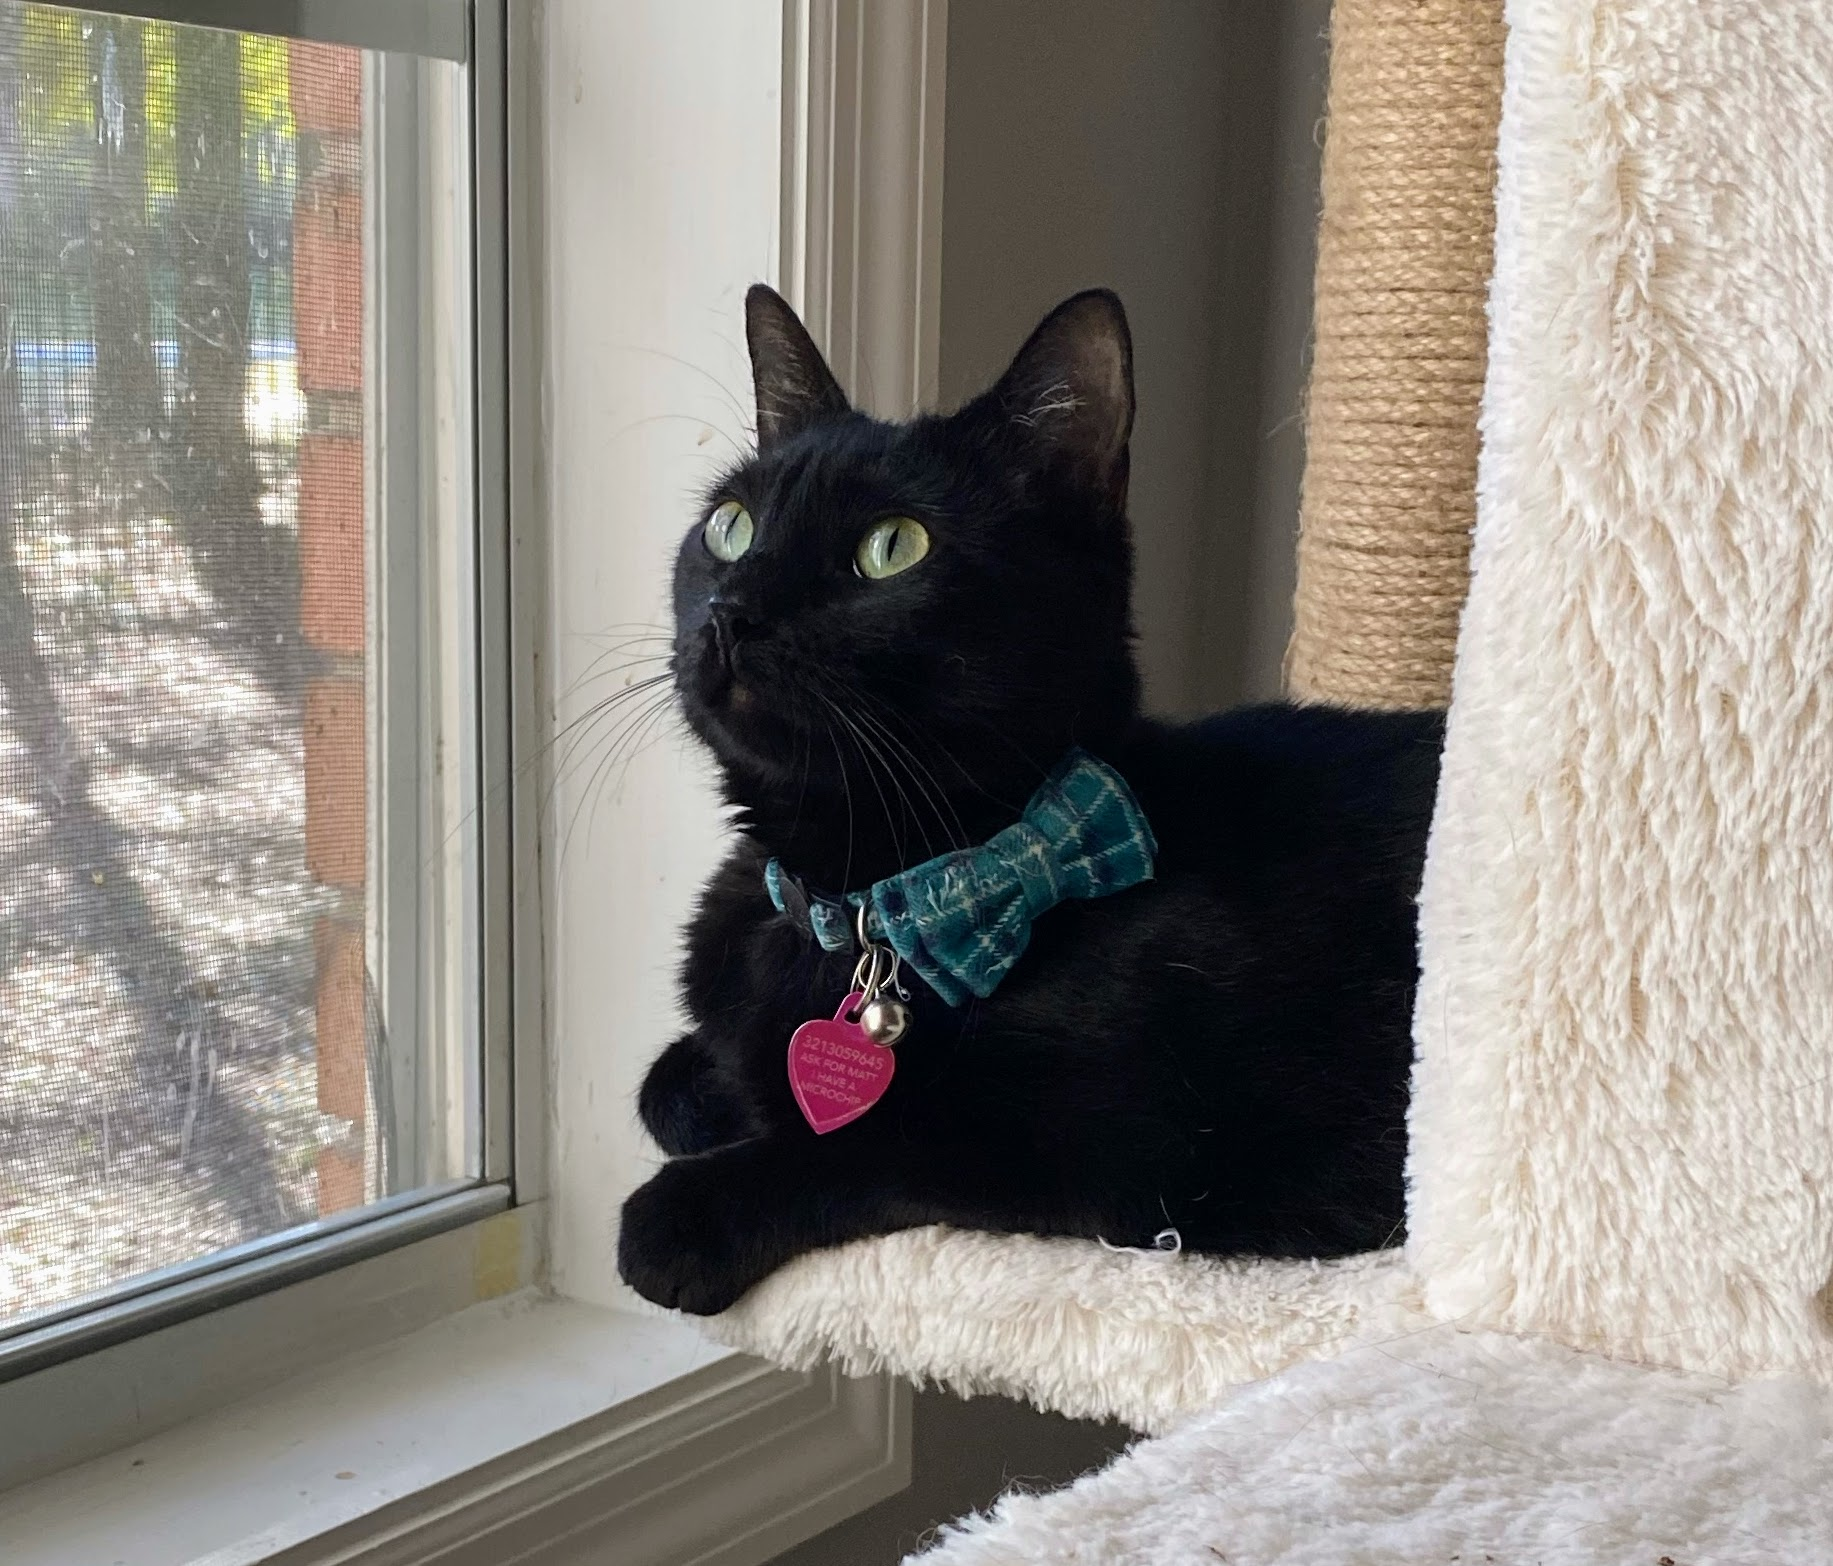
\includegraphics[scale=0.12]{bean.jpeg}
\end{center}



\tableofcontents


% %% The list of tables is optional. Remove the following line if you don't
% %% have tables, don't have many tables, or simply don't wish to have a list
% %% of tables.
% \listoftables


% %% The list of figures is optional. Remove the following line if you don't
% %% have figures, don't have many figures, or simply don't wish to have a list
% %% of figures.
% \listoffigures


% \chapter{Nomenclature, Symbols, Acronyms}

% The ``nomenclature, symbols, acronyms'' page is optional.


\chapter{Abstract}

% The ``abstract'' is required and is limited to 350 words.

The goal of this project is to provide a method of computer-enhanced performance to the solo clarinetist with minimal interference to their normal routine. The end goal if for a performer to be able to seamless switch between a traditional performance setting and an augmented one with a press of a button. Towards this goal, the Cyberinet is a hardware replacement for a portion of a clarinet containing a variety of sensors embedded within the unit. These sensors collect various real time data such as gyroscopic data of the performer and air flow within the instrument. This data is then transferred to a computer via Bluetooth connectivity in order to use the data in any number of potential electroacoustic performance settings. In addition to the base unit which is embedded within a 3D printed clarinet barrel, the Cyberinet was also designed to accept various expansion units through USB-C ports on the side of the device. This allows for the unit to become customizable based on various performance needs. The final portion of this project consists of a collection of Max objects designed from the ground up to utilize the Cyberinet’s data in musical contexts. These Max objects were utilized in the performance of three new compositions for the instrument on April 18th, 2023 in the Digital Media Center on LSU’s Baton Rouge campus.

%% The command ``\mainmatter'' switches to regular page numbers and
%% chapter headings that include the word ``Chapter''.
\mainmatter


\chapter{Introduction}
\label{chap:intro}
The practice of creating augmented musical instruments has been a method of creating new and unique timbres in musical performance for centuries. Some of the earliest instrument augmentations still in use today can be traced back to the early brass mutes of the 16th century. In the mid 20th century, John Cage developed a method for augmenting the possible timbres of the piano to vastly increase its sound-color-palette in compositions such as Sonatas and Interludes. 
As computer power has increased over the past 50 years,
computer processing has allowed for a more dynamic and varied application of instrument augmentation during live performance. As previously stated, the concept of altering an instrument’s method of performing and potential musical timbres has been around for several decades. In fact, this is a potential important step in the development of new instruments. 
Several works have been developed over the years towards this goal. Within the past 20 years, the Metasax and the Overtone Violin have been two instruments that fall into this category. These instruments take the mechanisms of performing on a alto saxophone and violin respectively, and build upon it to develop that instrument’s augmentation. The Metasax is built from a regular saxophone with various sensors built into the base instrument. These sensors allow for data to be collected and used to process sounds via an external computer. 
Unlike the Metasax, the Overtone Violin is built from scratch. This instrument replicates the violin in terms of form and sound production, but contains several internal pickups, sensors, and control buttons built into its form factor. In short, the various buttons can be used to adjust the performance modes and help adjust the data being collected and sent to a USB receiver located on a separate glove that the performer would wear. Bertner has written several pieces and performed in several conferences utilizing this instrument. \textit{Windsketches} (performed 2011) and \textit{Endprint} (2004) are two such compositions.

Both Of these instruments have something similar between them that this project is working to improve upon. That factor is that the performer must either acquire a completely new instrument or potentially permanently alter their instrument to perform with their augmented capabilities. They also require hard-wire connections in some regard, but this is less of a drawback in the context of this project. While these instruments do base their performance practices off of common instruments, there will have to be some level of re-learning the instrument in order to properly make use of its abilities. 
My project works to be minimally invasive to the performance practice of whomever is using the hardware. It is also designed to be easily added or removed to/from a performer’s instrument, eliminating the need for an additional instrument. Two projects that are designed to be minimally invasive are the MIGSI trumpet and the SABRe multisensor. These augmentations both attach to brass and woodwind instruments respectively. 

The MIGSI (Minimally Invasive Gesture Sensing Interface) trumpet is a collection of sensors that attach to the bottom of a trumpet. These sensors work to capture control data such as valve placement, instrument position, etc. and send it wireless to a computer. All of the sensors are positioned in a way that does not impede the traditional performance of a trumpet, although it does not appear to be something that can be easily removed in the moment if desired.
The creator of the MIGSI trumpet, Sarah Belle Ried, has created several improvisations utilizing the apparatus, and written several compositions such as Consider (2017). The SABRe is another sensor array that is designed to work with various woodwinds. The unit straps onto the instrument and can be used to collect airflow and position data to be wirelessly sent to a control computer. While effective and easily removable, this particular device offers a relatively limited amount of usable parameters which can be utilized in an augmented instrument. With the exception of an optional remote, this sensor is only able to utilize the sensors built into it, which include a gyroscope, accelerometer, thermometer, and airflow sensor.

These are all potentially useful, but if the performer does not need or want all of these, then they are stuck paying for the sensors that they will never utilize. The effectiveness of the SABRe Multisensor can be seen in compositions such as \textit{Sails} by Matthias Muller (2018). 
My project seeks to combine the best aspects from these projects and synthesize them into a new semi-modular design that any woodwind player can utilize. It takes the intention of using traditional performance practice to generate its augmentation, while still being something that can be adapted or easily removed in a performance based on the performer’s needs. My hardware is also something that does not impede the movements of the performer. In terms of form factor, My hardware takes inspiration from artist Pamala Z. when in use, one of her sets of sensors is located on her hands, and responds to various gestures to control her performances. Various iterations of these sensors can be seen in several of her compositions, including \textit{Breathing} and \textit{STEIM} (2007)
Taking inspiration from the SABRe, The Cyberinet's main hardware will be located on the instrument itself. This device will contain the majority of the sensors, batteries, and transmitters. To help with this, the instrument’s mouthpiece and barrel will be 3D printed as a housing for the embedded sensor, which will transmit its data via Bluetooth to a nearby computer.
Additional sensors can be connected to this unit via USB-C cables. These modular units are designed with the Pamala Z influence in mind. These sensors can be attached to various points on the body, instrument, or performance environment, and are intended to be easily adaptable for any performance setting.
Optional buttons can also be attached via wire to allow for additional performance control if desired. The wires connecting the optional units and the main hardware are all that is required for the Cyberinet. All of the data is wirelessly sent to the paired control computer. Where it will be utilized to augment the instrument sound and other elements.

\chapter{Historical Context}

\section{MIGSI Trumpet}
The Minimally Invasive Gesture Sensing Interface, or MIGSI Trumpet is an augmented instrument designed to work with the ergonomics and performance practice of the traditional trumpet\cite{reid2016}. Towards this goal, creator Sarah Belle Reid developed a collection of sensors that fit seamlessly into the form factor of the trumpet.

Where the MIGSI is similar to the Cyberinet is in its goals of form factor. The entirety of the MIGSI augmentations are located to match the form of a standard B-flat or C trumpet, and is placed at the instrument's center of gravity to minimize fatigue from the extra weight. While not as streamlined as the MIGSI trumpet, the Cyberinet's sensors are located in a similar location in relation to the design of the Clarinet.

\subsection{Music Written for MIGSI Trumpet}

Here we will discuss \textit{Pocket Fig} for the MIGSI Trumpet, written by Sarah Belle Reid\footnote{A performance video of \textit{Pocket Fig} can be found at \url{https://www.youtube.com/watch?v=5szWkbVjYxg}}. In this work, Reid utilizes Force Sensitive Resistors as well as Infrared sensors to collect data related to the valve displacement on the instrument. This data is then wirelessly sent to the computer to control a Max patch's granular synthesis processing.

\section{SABRe}
The SABRe is a system of sensors that is the device most closely related to the Cyberinet. Specifically comparing the two devices, we can see clear pros and cons to each.

\textbf{SABRe:}

\begin{itemize}
    \item Pros: small, completely wireless, easily removable.
    \item Cons: no modularity, cost.
\end{itemize}

\textbf{Cyberinet:} 

\begin{itemize}
    \item Pros: integrated within the instrument, expandable with add-ons, relatively inexpensive to produce, open source-components.
    \item Cons: less easily removable, some wires involved.
\end{itemize}

The core units of both devices contain a similar array of sensors. In fact, the SABRe was an inspirational starting point for the development of the Cyberinet. Both devices have a main unit containing the following sensors:

\begin{itemize}
    \item Gyroscope
    \item Accelerometer 
    \item Differential Airflow Pressure
    \item Temperature
\end{itemize}

From the similar sensors between the two different devices, one can infer a similar usage case as well. Both of the SABRe and the Cyberinet are add-ons for a clarinet. By being attached to the instrument, the sensors collect the data they are designed to collect and transmit it to a nearby computer.

The goal of the SABRe is to provide augmentation features to performers, regardless of their technical abilities\cite{Schiesser2012}.

As well as containing a similar base, the units also allow for an optional use of 2 buttons that can be programmed using the computer. However, it is at this point that the sensors begin to differ. It is the view of the author that the SABRe sensor is generally lacking in two main elements. The first is its lack of additional sensor options. While the included sensors are indeed quite useful for collecting performance data.

\subsection{Music written for the SABRe}

Prior to 2023, SABRe had been on a hiatus in terms of development and is currently in the process of designing a relaunch of the system. It is perhaps for this reason that there is a limited number of works for the system, but discussing the reasons behind the hiatus is beyond the scope of this paper.

One piece that will be discussed is  \textit{Sailing}\footnote{The performance of \textit{Sailing} can be found at \url{https://www.youtube.com/watch?v=Eiuacb5nJc8}} by the SABRe's creator: Matthias Mueller.  

In this work, Mueller takes the gyroscopic information from the SABRe to control audio effects in real time. The first one heard is the control of the amount reverb and delay time as the performer moves from right to left. This is followed by triggering a tremolo effect that combines with the clarinet timbre. Due to a lack of a score, it is my best guess from the video that this effect is being toggled on with the buttons located on the back of the instrument. By combing these effects with micro-tonal notes, Mueller is able to create a unique sound world easily and effectively.

Mueller also utilizes a pitch shifting effect, but it is unclear if it is created as a unique harmonizing effect, or is created as a by product of adjusting delay times. The final effect is a little distortion present when the performer reaches the extreme ends of the gyroscopic data.

In the future, should a performance score become available, it would warrant more in depth analysis of the performance practice and specific utilization of the SABRe's sensors. However, there is still much that can be learned with Mueller's performance video. It can be seen that Mueller clearly focusing on only one or two sensors present within the SABRe: Gyroscope and Buttons. By focusing on a smaller subset of the sensors, it allows Mueller to allow the capabilities to the system to stand out. It becomes very clear what the correlation between the clarinetist's physical position and the timbres being created are.

Mueller's utilization of the button is worth bringing up individually. in \textit{Sailing}, Mueller is using this button to trigger a tremolo-like effect to be applied to the clarinet's signal. Unfortunately without the software patch or score the fine details of this are left to speculation, but I want to focus on the idea of manually triggering an effect with a button. Unlike a foot pedal, these buttons follow the performer, allowing them to take full advantage of the buttons along with the movement sensors. A performer can access the buttons regardless of their on-stage location. In the Cyberinet compositions discussed later, I utilize a larger-scale use of the main buttons. In \textit{Puzzle of a Park}, the buttons are used to trigger recordings and playback, whereas in \textit{Raindrops on a Tin Roof} I utilize the button's instant binary functionality to cycle through different signal routing and effect presets to alter the tones.

\section{Other Similar Sensors}




\chapter{Intended Uses}

While widely adaptable, the Cyberinet was envisioned with a handful of specific uses in mind. As in, the Cyberinet is intended to be an easily-removable add-on for a standard B-flat clarinet.

\section{Composition Tool}
One of the main intended uses of the Cyberinet is as a compositional tool. Effectively, treating the Cyberinet as a completely new instrument or an add-on to a traditional B-flat Clarinet.

\section{Improvisation}
% a la stomp boxes

While mainly intended as a compositional tool, the Cyberinet leads to a large amount of exploration. Another use of the Cyberinet is in the practice of improvisation. A few audio effects are provided with the Cyberinet to allow for the user to easily begin creating their own sounds, however the system can easily send its data to any object within the Max environment. By exploring which sensors are connected to different audio effects, the performer can create a large number of sounds based on a single performance movement that they are already used to.

This modularity in signal processing is similar to the practice of using guitar stomp boxes to make a unique sound. While not physically similar, both systems allow for the quick customizable alteration of the instrument sound. When designing the available software objects, effects present in effect pedals such as reverb, delay, filters, and tuners were used as an inspiration.

% \section{Audience}

% This is a paragraph inside of a section.

% \subsection{Background}
% \label{sec:background}

% A paragraph in a subsection.

% \section{Citing bibliography entries, figures, tables, and }

% As shown in \cite{latexCompanion}, you
% can reference bibliography entries using the ``\verb|\cite|'' command.
% You can also refer to other parts of the document, such as
% Chapter~\ref{chap:intro} or \S\ref{sec:background}, but letting
% \LaTeX\ handle the numbering. That way, if you move things around, or
% choose a different numbering style, then you won't have to manually keep
% track of the changes.


\chapter{Cyberinet Hardware Components}

At its core, the Cyberinet contains a small collection of sensors build into the hardware. These include: [list of sensor names]. In addition to these sensors, the unit contain two USB-C connectors on its side. The first one is intended for the button board expansion, which gives the performer access to two buttons positioned on the thumb rest of their instrument. The functionality of these buttons can then be programmed using Max or another audio programming environment. The second USB-C port is designed to connect to a variety of other sensors, allowing for the performer to adjust their setup for whatever is needed for a particular performance. This is the origin of the phrase “semi-modular” in the project title. At the time of writing, one expansion sensor has been created and tested. This is the [figure something out, a mic that will respond to volume and transmit a bang.] Additional expansions have been planned and explored in more detail in the “Further Directions” section of this document. 
All these chips were selected for their ability to be dropped into the main board without an extensive need for the user to solder many components, and their use of standard 0.1 inch spacing. [fix this sentence]

\section{Micro-controller}
The ESP-32 DEVKIT was selected for a handful of reasons, including:

\begin{itemize}
    \item Board's narrow size
    \item Large number of ports
    \item Arduino compatibility
    \item Wireless communications
\end{itemize}

The first two items on the list are closely related. While being narrower that comparable Arduino units, the ESP-32 DEVKIT has 30 unique I/O Pins. While four pins are dedicated to power distribution and another for the 'enable' functionality (EN), the remaining 20 can be utilized for sensors in a variety of ways. All of this potential functionality is compressed to just 3 centimeters wide. Because of the ultimate physical design of the Cyberinet unit, having a large amount of accessible pins in a smaller unit was considered ideal. The DEVKIT was preferred over the significantly smaller base chip to increase the simplicity of prototyping, repair, and future changes due to its 0.1 inch pin spacing, and the popularity of the board among the community.

It should be noted that if using the ESP-32, but not the DEVKIT board, the number of available pins increases to 48, but the majority of these new pins are utilized for internal features. 

Because of the large number of Pulse-Width-Modulation-Controlled GPIO pins, the Cyberinet has the potential for a large number of sensors and expansions, but to help contain the form factor, only a handful are being utilized at any time. We can see the included sensors attached to the pins as shown below. More details about each of the sensors are discussed in each of the following sub-chapters. The labels in the figure below utilizes the pin labels that are printed on the DEKVIT. (look at pic for GPIO number)

\begin{itemize}
    \item VIN: Power from Battery
    \item GND: Ground
    \item 2: Power LED
    \item 4: Togglable LED
    \item 12: Button 1
    \item 14: Button 2
    \item 21: Gyroscope and Airflow Data
    \item 22: Gyroscope and Airflow Clock
\end{itemize}

Both the Gyroscope and Airflow pressure sensors utilize the same pins. These are the I2C pins on the DEVKIT. More details will be discussed in the chapter discussing the Arduino programming, but it should be noted now that these sensors are able to utilize the same pins because they utilize different I2C addresses. The code is able to access these different addresses in sequence when collecting data.

The code written for the ESP-32 DEVKIT was created using the Arduino IDE and coding language. For similar reasons to the choice of the DEVKIT, this was done for greater accessibility and simplicity in programming. More details about the Arduino Code are discussed later, and the code as a whole is included in the appendices.

The final item from the initial list was the wireless capabilities. The ESP-32 is able to perform serial communications with a connected computer via a micro-USB or USB-C cable (depending on the board version). While useful, the goal of the Cyberinet is to provide affordable instrument augmentation with minimal alterations to the clarinetist's performance practice. Towards this goal, minimizing the number of extra cables was a design concern from the first prototypes. By utilizing the built-in Bluetooth capabilities, the performer is able communicate with the computer easily while meeting this requirement.

The ESP-32 also has WiFi connectivity capabilities which may be involved in a future version, but at the current time is currently not utilized. The DEVKIT is able to support Bluetooth version 4.2 and Low Energy protocols for local wireless communication. This allows for the Cyberinet to easily pair with any computer that it has previously connected to using the BTSerial Arduino library. A code library that brings the normal wired Serial functionality to the Bluetooth functionality.

While not as powerful as the most up-to-date Bluetooth hardware, the DEVKIT's version 4.2 allows the Cyberinet to connect to a computer from up to 200 feet away with a max data transfer speed of 1 Mbps. While these values do fluctuate depending on the performance venue layout, and have a minor impedance from the case of the Cyberinet itself, the performance statistics are still high enough for a large majority or performance areas. This will be discussed more in the chapter discussion the music compositions and performance with the Cyberinet.

\section{Gyroscope \& Accelrometer}
MPU-6050


\section{Power Distribution}
TP-4056 Type C
The TP-4056 is a standard chip utilized for the charging of lithium ion polymer batteries. This variant utilizes a USB type C connector over the micro-USB connector of the base model and allows for both the charging of the battery as well as the distribution of power from that battery. When charging, it is the USB-C port that is connected to the power supply. As seen in the hardware diagrams, no other USB-C port is directly connected to this chip.

\section{Differential Airflow Pressure}

SDP-31
Originally released in [year], this is the newest hardware component in the Bill of Materials. This unit detects differential airflow pressure between two points as well as temperature. Due to the SDP-3X line’s small form factor, the Sparkfun Qwiic connector break out board was selected for simple installation. Two small tubes are attached to the ports and used to measure the air pressure difference between the inside of the clarinet mouthpiece and the outside of the instrument.
Because of it’s higher accuracy, the SDP-31’s temperature sensor is utilized over the MPU-6050. Temperature is measured in degrees Celsius.

\section{LiPo Battery}
In order to power the entire system, a lithium ion polymer battery is included inside the hardware. In order to charge the unit, users can utilize the provided USB-C cable and power adapter to the port located on the bottom of the unit [show picture]. From an empty charge, the unit can take between one and three hours to fully charge. The exact times can vary depending on the power adapter and whether any additional accessories are connected. 
The Battery included is rated for 1200 mAh as an improvement over the 320 mAh battery used for initial testing and prototyping. This size battery allows the Cyberinet to have as much run time as possible while still maintaining the size characteristics of the hardware electronics. The approximate run times are as follows:

\begin{itemize}
    \item Powered on, not connected: 4 hours.
    \item Powered on, Bluetooth connected, no expansions added: 4-5 hours.
    \item Powered on, Bluetooth connected, expansions added: 3 hours.
\end{itemize}


It should be noted that the device can also run when connected directly to the wall socket power supply. This will also charge the battery, which, while resulting in yet another wire, can result in an indefinite run time.

When the battery capacity becomes critically low, the device will stop transmitting data, however the LEDs may stay on due to residual amounts of electricity present in the system. To avoid accidental drop outs during a performance, it is recommended to fully charge the device prior to any performances to avoid this. When the battery reaches 20\% charge, the red LED on the device will illuminate, and then flash as shown below:

\begin{itemize}
    \item 15\%: 1 flash
    \item 10\%: 2 flashes
    \item 5\%: 3 flashes
\end{itemize}

[have the device auto power off? Look into doing that at 2%] More information about how the Cyberinet responds to internal battery levels can be found in the software discussion portion of this document.


\section{Button Board}

These attachments are optional and not needed for the Cyberinet main unit to be functional and are intended to only be connected when needed for a particular performance. All the expansions connect utilizing a standard USB-C connector. However, these units do not utilize the USB protocol, so both the main unit and expansions cannot be connected to a computer via these ports. Because the Cyberinet does not communicate to these using USB protocol, not all USB-C cables can be used for this, however the vast majority can. [make this true] While a set of USB-C cables that are functional is included with the full Cyberinet set of hardware, The main reason for utilizing this connector is for the end-user to be able to supply their own cables of various lengths depending on their needs. 

This board, while optional, is incredibly useful for a performer on stage. They can access the buttons using their right thumb when performing. This maneuver is easier when utilizing a neck strap, so the performer can place the buttons elsewhere if they like using a longer connector cable. Each button also contains a single, colored LED built into it to provide feedback to the performer. By default, the lights are only illuminated when the button is pressed. [investigate a way to change that perhaps?] The Cyberinet simply detects whether a button has been pressed and transmits that data as a Boolean value to the computer. Using a program such as Max, the user can have the buttons achieve functions from near limitless hypothetical list of options. For this project, the buttons were used to trigger microphone recording and buffer playback, however objects that take the button input and move between various presets, trigger DSP, and turn pages of a score have also been developed and included in the software bundle for this project.

\chapter{Physical Design}
This chapter discusses the physical characteristics of the Cyberinet.

\section{Main Body}

The main unit of the Cyberinet is designed to replace the uppermost portions of a B-flat clarinet: The barrel and mouthpiece. As shown in th image, the electronic components are housed in the box on the performer's right side of the instrument. Placing the electronics here allows for the unit to be easily adjusted for tuning or be easily removed as needed. The box was made as small as possible, but it still contains all of the electronic components except the button board and any other external add-on components. Because of this size restriction, a small ligature is provided along with the Cyberinet in the event that the box would interfere with the performer's normal ligature.

The aforementioned ligature, electronics housing, and replacement barrel/mouthpiece are all 3D printed using a black Polylactic acid (PLA) material. Other materials were considered, but the PLA allows for both a consistent sound and affordable printing of the units.


\section{Button Board}


\chapter{Software}
This chapter discusses the code located within the Cyberinet itself, as well as the accompanying library of Max tools. Discussion of the software portion of each of the included music compositions will be discussed in that chapter. 

\section{Arduino Code}

\section{Max Library}

To utilize the data being collected by the Cyberinet’s hardware, I have created a small library of Max objects to help with the collection and usage of said data. While detailed below, it is important to mention that Max is a paid software. The software and hardware components are all open source, however in order to create your own patches, the end-user will need to download the software. If saving patches is desired, then they must purchase a software license. Potential freeware options are being considered and will be explored upon more in a later chapter, but at the time of writing, are not in active development.

The main core of the Max library consists of two main objects. These are the .receive and omnirecieve objects respectively. Looking at the former of the two, This object is designed to receive serial data from the Cyberinet, but filters out all data except that from a given sensor. This is useful for scenarios when the full functionality of the Cyberinet is not needed. omnireceive, as the name implies, receives data from the Cyberinet as well and outputs the data from each sensor to unique outputs. This allows for the user to easily access any of the incoming data at once, and is useful for prototyping which sensor control could be useful for ran effect, or in a performance scenario when multiple sensors are required.

While not necessary for the functionality of the Cyberinet, I have also created a small collection of Max objects for use with the unit. These objects were all used within the Compositions discussed in chapter 7. All of these objects are designed from the ground up to receive data from the Cyberinet in order to control their functionality. These include:

\begin{itemize}
    \item Reverb: a Schroder style reverb based on examples from CCRMA.
    \item Compressor: Based on the compressor objects created by Cycling74.
    \item Simple Delay: A single delay line using the tapin~ and tapout~ objects. 
    \item Multi-Delay: A delay line utilizing 4 different tapout~ objects to create multiple delay lines. Each one can have its individual output level set for unique mixing capabilities.
    \item Feedback Delay: Identical to the simple delay, but with a feedback option added.
    \item Vibrato Delay: Functions similar to the Simple delay object, but includes a basic implementation of FM synthesis to adjust the pitch of the signal to be delayed. 
    \item Tuner: This object functions like most other tuners available on the market. It will determine the pitch of an incoming signal and display its equal temperament tuning visually on the screen. This is useful for checking and maintaining tuning within the Max environment, and for having the Max patch respond to certain pitches. This object requires a microphone be used to monitor the input as the ADC capabilities of the ESP-32 DEVKIT are unable to pull off this effect
\end{itemize}

In addition to the above objects, the Cyberinet software also includes a few objects intended to be helpful in setting up and trouble shooting. The main one of these objects is the tuner object. This object serves as a tuner within the Max environment, allowing for quick adjustments to be made without needing an additional piece of hardware. 
The main downside to the tuner object is that it requires the use of a microphone input to the computer. This is due to the limited ADC capabilities on the Cyberinet's main ESP-32 Board. However, an unexpected upside to the object is it's pitch detection capabilities. The tuner object is able to detect both the musical pitch of the incoming signal, but also fine tuning in cents. Because this information is expressed in MIDI, it can be used to trigger a variety of other events in the max environment. While the list of possibilities is extensive, the idea of having the max patch harmonize with the clarinet is one of particular interest to the author.

[tutorial and help patches]
[make it into a standalone program? Maybe if there is time, maybe as a future endeavor]

\chapter{Music Works Written for the Cyberinet}

In addition to creating the hardware and software for this dissertation, I have also created a handful of musical compositions that show off various features of the Cyberinet. These three compositions as listed below, show a gradient from simpler to more complex uses of the Cyberinet’s features.

\section{Puzzle of a Park}
At its core, this work is the simplest of the three written especially for this project. \textit{Puzzle of a Park}\footnote{A performance video of \textit{Puzzle of a Park} is available at} functions as a work written for a loop pedal, but without the pedal. The performer plays through the material from beginning to end, periodically pressing one of the two buttons on the button board accessory. Looking at the max patch we can see that one button will trigger the computer to record a microphone input into a buffer while the second triggers the synchronized playback of all recorded buffers. 
[show patch snapshot]
This functionality allows for multiple recordings to be saved and layered, much like loop pedals such as the Boss RC line of pedals. [do I talk about multi tracking?]
When writing this work, I viewed the musical content as a quartet, with four unique voices rather than a single voice repeated several times. This allowed the musical content to flow and feel more organic once the final layer was added. 
Once I had completed the short musical section, it was simply a matter of repeating the sequence of time signature and meter changes so that the score would form a repeating pattern. From there I had to decide exactly how to organize the sounds in time. Because I wanted this to be the simplest of the works in terms of performance and programming, I refrained from breaking down the recordings into smaller chunks and assembling them in Max. Instead, I choose the loop pedal approach and had the performer play through each voice before starting the playback and recording for the following voice. 
When ordering the voices, I began with one of the middle voices as the opening to the solo part. When comparing the voices in the score, these helped to provide a large amount of the background and a steady, albeit syncopated, pulse to the music. Something that helps to give the following bass voice more context during the measures where it is simply holding a pedal tone during the second section. Looking at the large-scale musical form of the solo, I would describe it as \emph{ABA'C} since the third and first voice are often coordinated, providing harmonic content. I viewed them like a horn part in a Sousa march in this regard. When combined, the first three voices provide a complete backing track to the main melodic line. Like fitting together, the pieces of a puzzle, it is this final line that helps to give context to all the phrases we have heard so far. Down beats become upbeats, harmonic implications shift with the addition of new chord tones, and the texture is filled out to include the full range of the instrument.


\section{Ethereal Presence}
The second work\footnote{A performance video of \textit{Etherial Presence} is available at} created for this project begins to utilize the more complicated sensors present in the Cyberinet. These primarily include the gyroscope and airflow meter. Once received, the Max patch for the composition utilizes the values to control two different synthesizers and their parameters. 
[chart showing the value and parameter mapping]
The first synthesizer outputs a single tone with the goal of harmonizing with the soloist. This is the Ethereal Presence as mentioned in the title. [add more when this synth is done]
Accompanied by this is a more textural synthesizer designed to help support and fill out the atmosphere of the composition. This synthesizer outputs noise before being run through an FFT, based filter created by Dr. Austin Franklin [ how much info on the project do I need?]. This filter takes the incoming noise and performs an FFT operation on it to determine the frequency content, then based on the values received from the Cyberinet, filters out certain frequency bins. 


\section{Raindrops on a Tin Roof}
Of the three debut compositions for the Cyberinet, \textit{Raindrops on a Tin Roof}\footnote{A performance video of \textit{Raindrops on a Tin Roof} is available at} is the most involved with the Cyberinet sensors. Contrasting from Mueller's usage of the SABRe, this composition utilizes all of the default sensors present in the hardware in some way. 

The inspiration comes from a short story [summarize the text here]

Formally, the music follows the narrative of the story, with ambient storm sounds and monster noises coming in as indicated. 

Gyroscopic information is used to control the live mixing of the pre-rendered tracks. These include:
\begin{itemize}
    \item Two different storm ambience tracks.
    \item Sounds created by the monster.
    \item Creaking floorboards.
    \item Synthesizer Accompaniment.
\end{itemize}

The gyroscopic information is also used to alter effects applied to all of the aforementioned sounds as well as the clarinet. This is combined with the accelerometer information to avoid having the correlation become predictable.

The airflow information is used to apply distortion and other processing to the audio signals. In short as the performer's breathing increases, so does the effect application.

Unlike the other compositions discussed here, \textit{Raindrops} utilizes notated accompaniment. This accompaniment is meant to represent the monster in the basement in a less literal sense. For the premiere, these sounds are generated with the UVI 8-Bit Synth. This instrument is loaded into the Max environment using the vst~ object and is intended to create a spooky, slightly incongruous sound when compared to the other sounds in the environment. 
The musical content for this synthesizer was generated using the MIDI information from the notation software that created the score. Instructions for generating your own audio clip for this voice are indicated in the score. This freedom allows for the performer to create a timbre and environment that is unique to them.

\chapter{Future Directions}

In general, the Cyberinet has a few areas for future expansion. These can be broken into two main categories: instrument compatibility and functionality expansions. 

\section{Instrument Compatibility}
At the time of writing, the Cyberinet is only available for B-flat soprano clarinets. While this is the most commonly found Clarinet, it represents only a fraction of the total woodwind family. In the future, plans to adapt the hardware case to fit different instruments will allow for the Cyberinet to be utilized in an exponentially larger number of scenarios. 
First, adapting the unit for the A Clarinet and Bass Clarinets. At this time there are no plans to expand to an E-flat Clarinet due to the limited space to attach electronic components.
Following the Clarinet expansions, ideas for compatibility with Saxophones and Flutes are being discussed, but require more planning in order to make functional units.

\section{Functionality}


\subsection{Hardware}
Outside of the aforementioned hardware needed to make the Cyberinet framework compatible with more instruments, an increase in modular expansions is also planned. Initially only additional buttons and a volume-sensing microphone are available, but plans for the following sensors to be released in the future have been made:

\begin{itemize}
    \item Pressure Sensor: responds to varying pressure on the instrument's keys. Needs special mounting of Force-Sensitive-Resistors, as well as doughnut-shaped FSRs.
    \item Pitch Detection: Works like the tuner software object. This will display tuning information and transmit pitch information to the computer. Needs hardware with adequate Analog-to-Digital Conversion.
\end{itemize}

\subsection{Software}
Lastly, Plans for the expansion and revision of the software environment are already underway. Future goals include:
\begin{itemize}
    \item Adapt messages to OSC formatting for a greater range of software compatibility.
    \item Revising the current collection: small tweaks to improve appearance and functionality.
    \item Increasing Effects: Expanding for additional audio effects. Plans include filters, synthesizers, and automatic harmonizers.
    \item Troubleshooting \& Help Patches: While the current software environment contains help patches, in the future this area will be expanded and improved in a manner similar the the aforementioned revisions.
    \item Max Library: Once fully expanded, Plans to reach out to Cycling74 to have this collection of Max objects listed in the program as an available-for-download library will be made. This will make it simpler for people to access various tools for their Cyberinet unit.
    \item Standalone Software: The final planned software expansion is to take the Max environment and export it as a standalone software. This will allow for the user to access the tools and capabilities of the Cyberinet without needing Max, which can be a financial hindrance to some people.
\end{itemize}



%% The command ``\appendix'' switches into appendix-mode, meaning that subsequent ``\chapter'' commands will instead produce appendices.
\appendix

\chapter{Cyberinet Hardware Resources}
This appendix contains images for all of the 3D models and PCBs used within the Cyberinet. It also contains close-up images of each of the individual OEM sensors.

\section{3D models}
Below are all of the 3D models utilized to 3d print the case and accessories of the Cyberinet

\subsection{Main Body}
\vspace{5mm}


\subsection{Button Board}
\vspace{5mm}


\subsection{Accessories}
\vspace{5mm}


\section{PCB Diagrams}
Below are the PCB diagrams for the Cyberinet.

\subsection{Cyberinet Main Unit PCB}
\vspace{5mm}

\begin{center}
    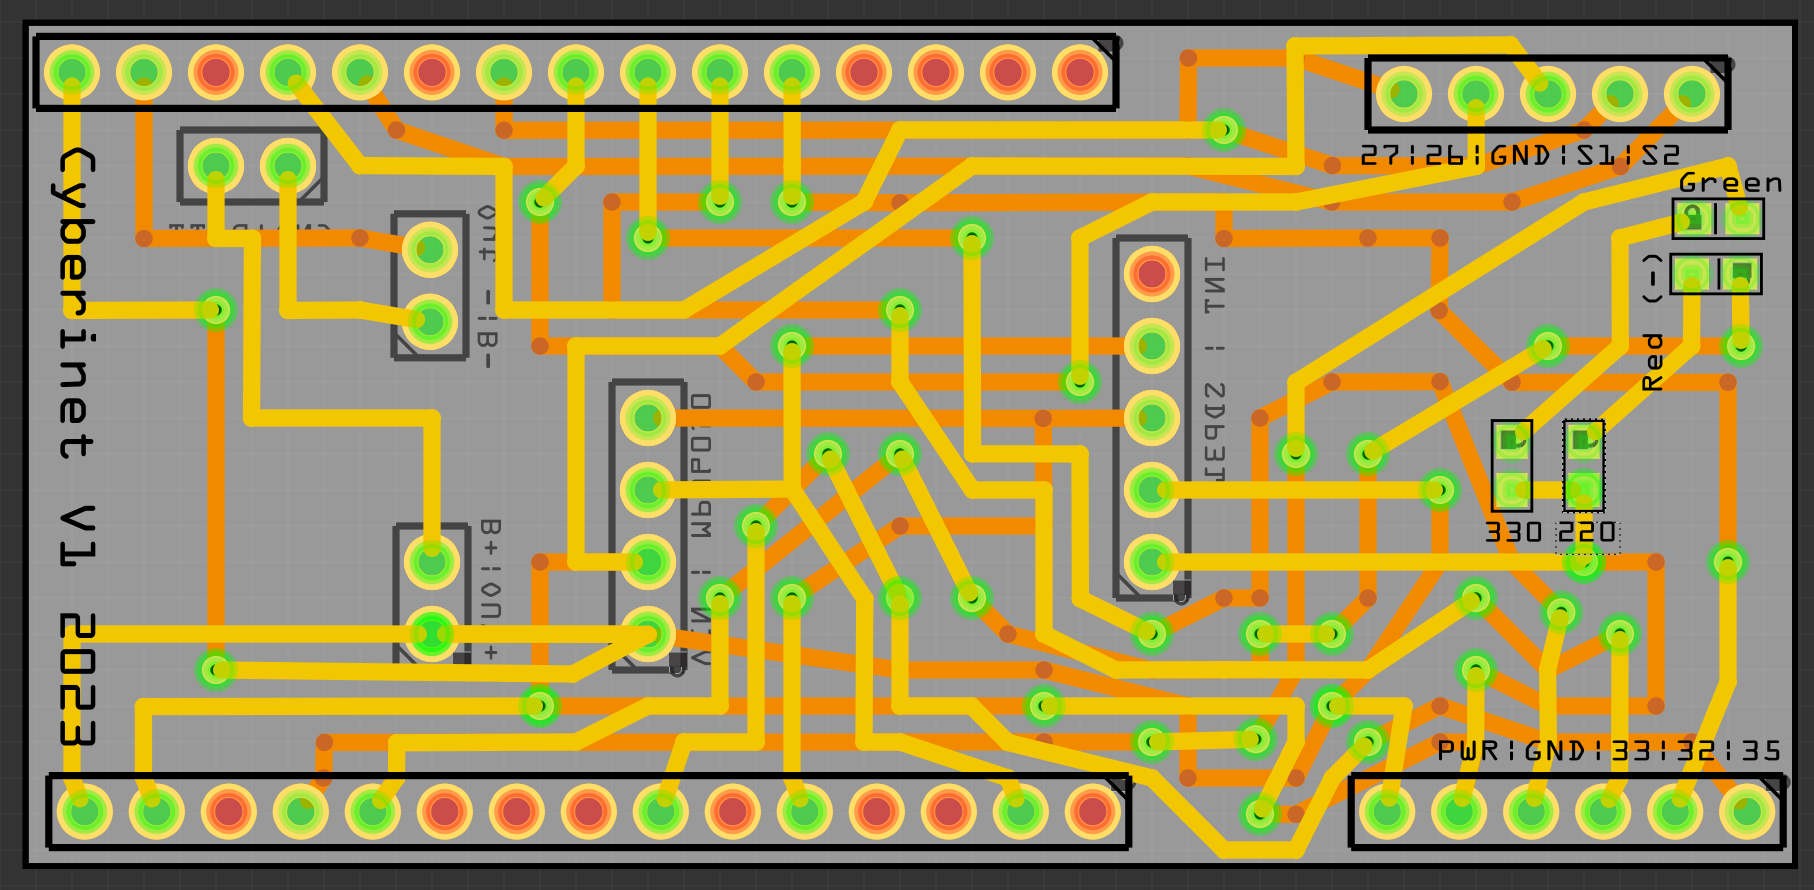
\includegraphics[scale=0.5]{diagrams/PCBs/mainBoard.png}
    \caption{Main Board Top View}
\end{center}

\subsection{Button Board}
\vspace{5mm}

\section{Sensor Chips Detailed Photos}

\subsection{ESP-32}
\vspace{5mm}

\subsection{SDP-31}
\vspace{5mm}

\subsection{MPU-6050}
\vspace{5mm}

\subsection{TP-4056 Type C}




\chapter{Cyberinet Software Components}
This appendix contains all of the Arduino code flashed to the Cyberinet. (Version 1), as well as screenshots of the various max patches and objects included in the software bundle.

\section{Arduino .ino Code}

\section{Max Objects}

\subsection{Functional Objects}

\subsubsection{receive~}
\vspace{5mm}

\subsubsection{omnireceive~}
\vspace{5mm}

\subsubsection{tuner}
\vspace{5mm}

\subsection{Audio Effects}


\subsubsection{reverb}
\vspace{5mm}

\subsubsection{delay}
\vspace{5mm}

\subsubsection{feedback delay}
\vspace{5mm}

\subsubsection{multi delay}
\vspace{5mm}

\subsubsection{vibrato delay}
\vspace{5mm}

\subsubsection{compressor}
\vspace{5mm}

\subsubsection{karplusStrong}
\vspace{5mm}



\chapter{Puzzle of a Park Score}

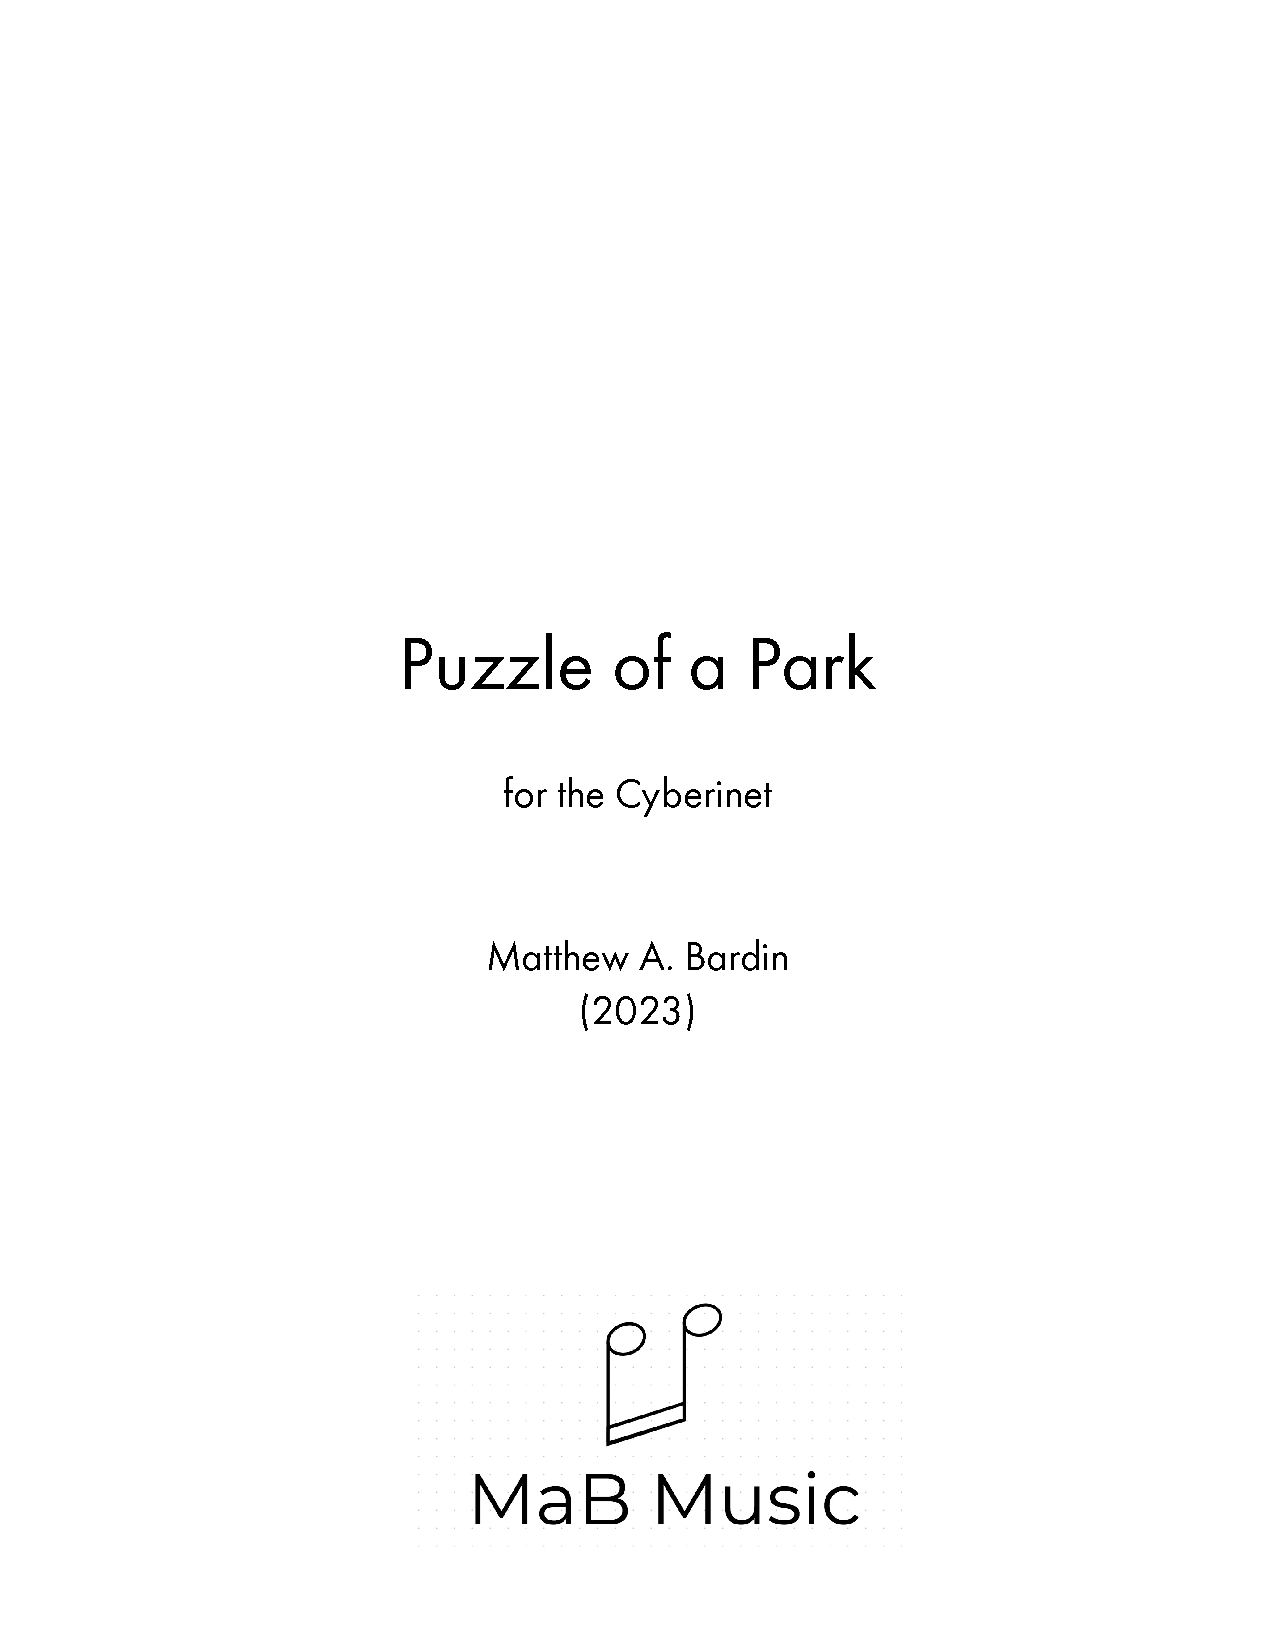
\includepdf[pages=1-17]{Scores/PPFull.pdf}

\chapter{Ethereal Presence Score}

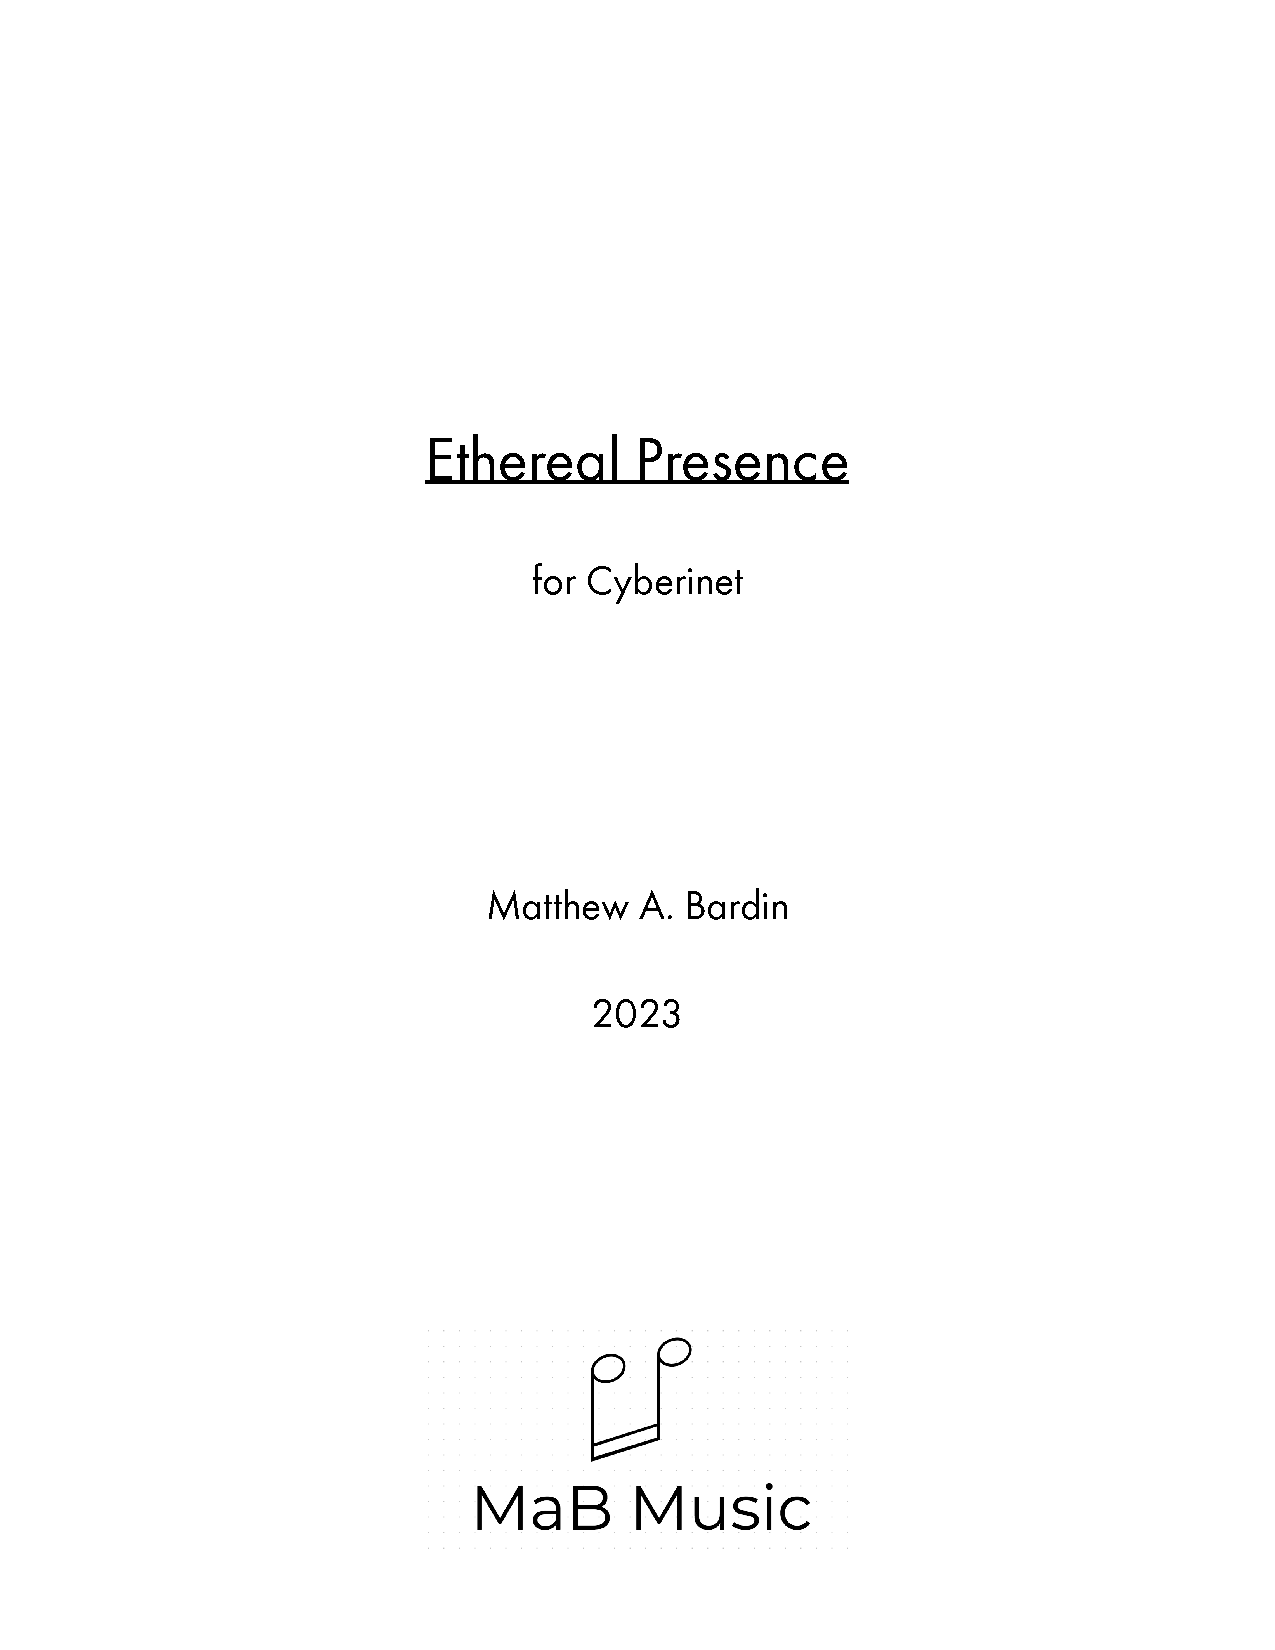
\includepdf[pages=1-9]{Scores/EP.pdf}

\chapter{Raindrops on a Tin Roof Score}

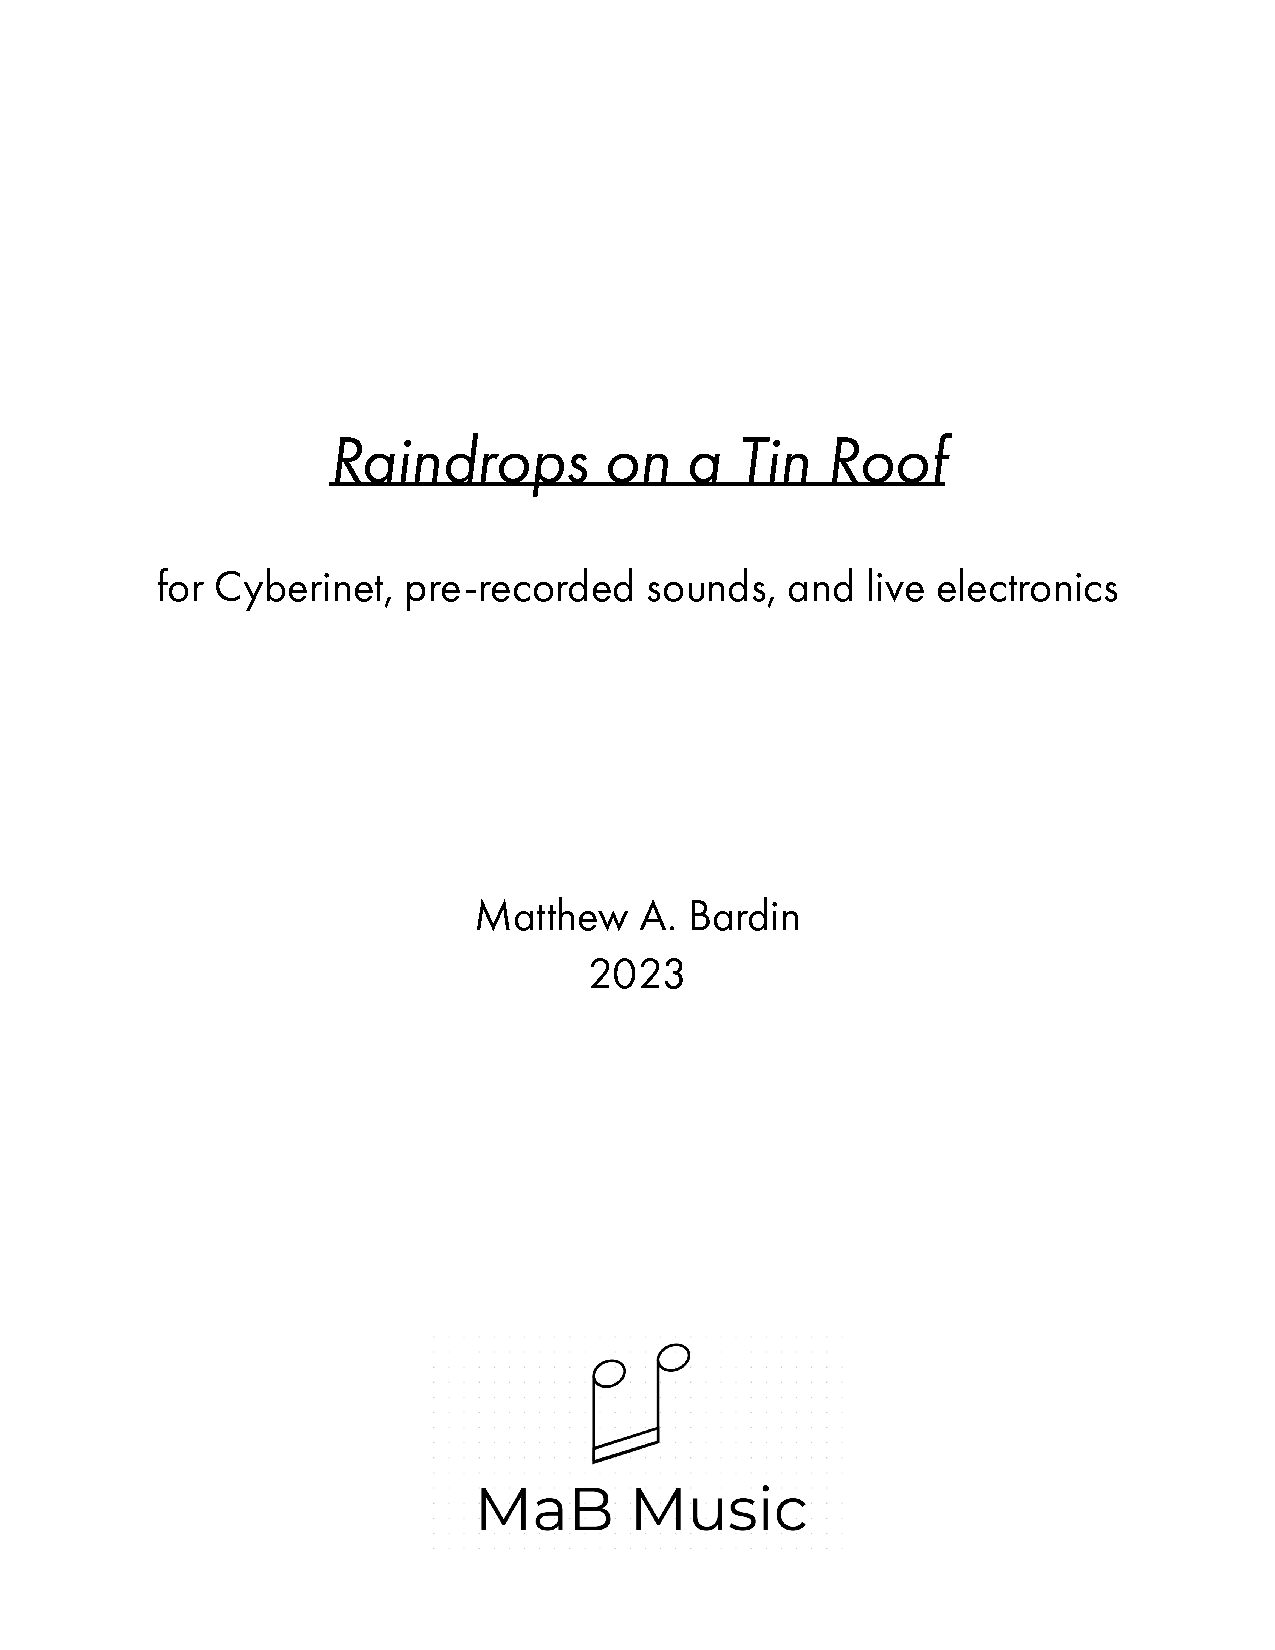
\includepdf[pages=1-8]{Scores/raindrops.pdf}
%  list page range and file location

\chapter{Raindrops on a Tin Roof Short Story}

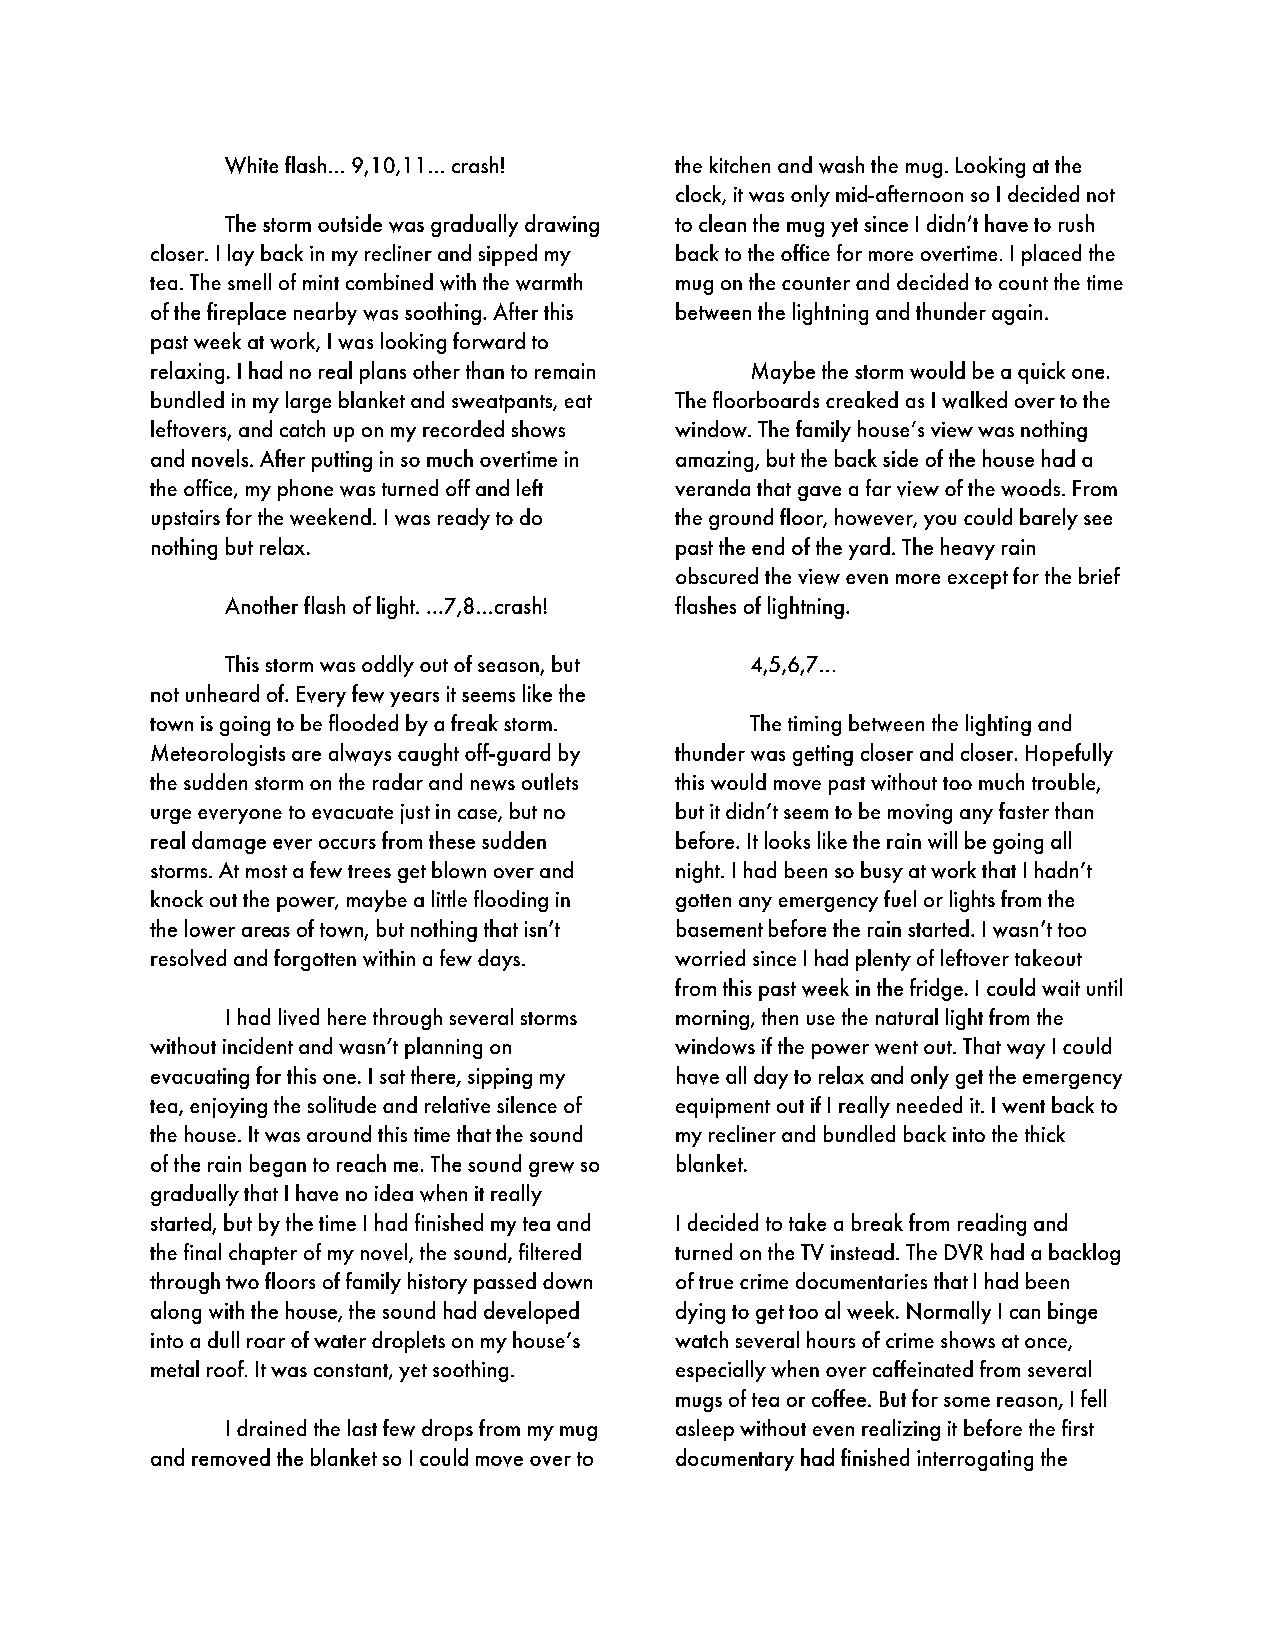
\includepdf[pages=1-4]{Scores/Raindrops Text.pdf}



% \chapter{Permissions}

% The ``permissions'' area reproduces requests and permissions for previously published material or material belonging to others. If included, then it should be the last appendix.


%% After ``\backmatter'', subsequent \chapter commands produce
%% unnumbered headings.
\backmatter


\begin{thebibliography}{99}

\bibitem{puzzleScore} Bardin, Matthew. \emph{Puzzle of a Park} Performance Score, MaBMusic, 2023.

\bibitem{EPScore} ---. \emph{Ethereal Presence} Performance Score, MaBMusic, 2023.

\bibitem{Raindrops Score} ---. \emph{Raindrops on a Tin Roof} Performance Score, MaBMusic, 2023.

\bibitem{Raindrops Score} ---. \emph{Raindrops on a Tin Roof} Short Story, Kindle Direct Publishing, 2022.

\bibitem{reid2016} Reid, Sarah and Gaston, Ryan and Honigman, Colin and Kapur, Ajay. \emph{Minimally Invasive Gesture Sensing Interface (MIGSI) for Trumpet}, Proceedings of the International Conference on New Interfaces for Musical Expression, 2016.

\bibitem{Schiesser2012} Schiesser, S{\'e}bastien and Schacher, Jan C. \emph{SABRe: The Augmented Bass Clarinet}, Proceedings of the International Conference on New Interfaces for Musical Expression, 2012.



% look at a way to make this better. I HATE how the template is handling references.


% \bibitem{mathIntoLatex} George Gr\"{a}tzer,
% {\em Math into \LaTeX: an introduction to LaTeX and AMS-LaTeX, Third Edition},
% Library of Congress, Boston, 2000.

\end{thebibliography}


\chapter{Vita}

Matthew Bardin, originally a native of Central Florida, is currently based in Baton Rouge, and has written music for large ensembles, chamber groups, voice, solo instruments, and electronics. He holds a Master of Music from the Boston Conservatory at Berklee, and a  Bachelor of Music from Stetson University. Matthew is currently working towards a Ph.D in Experimental Music \& Digital Media from Louisiana State University. He is currently affiliated with the American Society of Composer, Authors, and Publishers. His works are often performed by several student soloists and groups throughout the course of the academic year. He also has presented his music at the annual Electric LaTex festival, co-hosted an online workshop at NIME 2020, and served as the 2021 Composer in Residence of the University Presbyterian Church in Baton Rouge, LA. In 2022 he traveled to Edinburgh, Scotland to run audio for the LSU produced show \textit{Dream Logos}; a show for which he also composed the music and sound design.

Matthew has studied with Drs. Sydney Hodkinson, Eun Young Lee, Tina Tallon, and most recently, Drs. Jesse Allison, Edgar Berdhal, and Mara Gibson. Recently, Matthew has completed the audio for Dream Logos, an experimental physical theatre production with the the LSU Theatre program in Edinburgh Scotland. Matthew is currently teaching the courses Sound Design, Digital Storytelling, and Programming Digital Media to local dual enrollment students through the LSU STEM Pathways Program. The last of which, Matthew has written a large portion of the course textbook.

\end{document}
